\documentclass[aspectratio=169, 12pt]{beamer}

% --- Modern Professional Theme ---
\usetheme{CambridgeUS}
\usecolortheme{dolphin}
\setbeamertemplate{navigation symbols}{}
\setbeamertemplate{headline}{} % Remove top bar/line

% Professional color scheme
\definecolor{darkblue}{RGB}{0,51,102}
\definecolor{mediumblue}{RGB}{51,102,153}
\definecolor{lightgray}{RGB}{245,245,245}
\definecolor{accentgold}{RGB}{184,134,11}

\setbeamercolor{structure}{fg=darkblue}
\setbeamercolor{frametitle}{bg=white,fg=darkblue}
\setbeamercolor{title}{bg=darkblue,fg=white}
\setbeamercolor{block title}{bg=mediumblue,fg=white}
\setbeamercolor{block body}{bg=lightgray,fg=black}

% Custom footer with blue bar showing frame title
\setbeamertemplate{footline}{
  \leavevmode%
  \hbox{%
  \begin{beamercolorbox}[wd=\paperwidth,ht=2.5ex,dp=1ex,leftskip=.3cm,rightskip=.3cm plus1fil]{footline}%
    \usebeamerfont{footline}\insertframetitle\hfill\insertframenumber{} / \inserttotalframenumber
  \end{beamercolorbox}}%
  \vskip0pt%
}
\setbeamercolor{footline}{bg=darkblue,fg=white}

% --- Packages ---
\usepackage{booktabs}
\usepackage{caption}
\usepackage{graphicx}
\usepackage{amsmath}
\usepackage{amssymb}
\usepackage{tikz}
\usepackage{tcolorbox}
\usepackage{xcolor}
\usepackage{hyperref}

% Custom box for key points
\newtcolorbox{keypoint}{
  colback=lightgray,
  colframe=mediumblue,
  boxrule=1pt,
  arc=3pt,
  left=5pt,
  right=5pt,
  top=5pt,
  bottom=5pt
}

% Section slides
\AtBeginSection[]{
  \begin{frame}
  \vfill
  \centering
  \begin{beamercolorbox}[sep=8pt,center,shadow=true,rounded=true]{title}
    \usebeamerfont{title}\insertsectionhead\par%
  \end{beamercolorbox}
  \vfill
  \end{frame}
}

% --- Metadata ---
\title[Design of VAE for Indic Scripts]{Design of Variational Autoencoders for Indic Scripts}
\author[K. Sarma \& R. Pamidi]{
    \textbf{Karthik M Sarma} (S20230030385) \\
    \textbf{Rohit Pamidi} (S20230030398)
}
\institute[IIIT Sri City]{
    Bachelor's Thesis Project \\
    Indian Institute of Information Technology, Sri City \\
    \vspace{0.2cm}
    \textbf{Guide:} Dr. Pavan Kumar Perepu
}
\date{February 2026}

\begin{document}

% --- SLIDE 1: Title ---
\begin{frame}
    \titlepage
\end{frame}

% --- SLIDE 2: Individual Contributions ---
\begin{frame}{Individual Contributions}
    \begin{columns}
        \column{0.48\textwidth}
        \textbf{Karthik M Sarma:}
        \begin{itemize}
            \item Performed complete primary data collection 
            \item Assisted in presentation preparation and design
            \item Authored and completed the written report
        \end{itemize}
        
        \column{0.48\textwidth}
        \textbf{Rohit Pamidi:}
        \begin{itemize}
            \item Implemented affine transformations for Telugu dataset
            \item Designed presentation structure and planning
            \item Conducted comprehensive literature review
        \end{itemize}
    \end{columns}
\end{frame}

% --- SLIDE 3: Outline ---
\begin{frame}{Outline}
    \tableofcontents
\end{frame}

% ========================================
% SECTION 1: INTRODUCTION
% ========================================
\section{Introduction}

% --- SLIDE 4: Introduction ---
\begin{frame}{Introduction}
    \begin{columns}
        \column{0.55\textwidth}
        \textbf{Indic Scripts \& Akshara:}
        \begin{itemize}
            \item \textbf{Akshara:} Fundamental writing unit in Indic scripts - represents syllables rather than individual phonemes
            \item \textbf{Brahmi script family:} Ancient writing system originating from Brahmi script (~3rd century BCE)
            \item \textbf{Telugu script:} Dravidian language family, ~75 million speakers, rounded characters
            \item \textbf{Devanagari (Hindi):} Indo-Aryan language family, ~600 million speakers, horizontal line at top
            \item \textbf{Script characteristics:} Non-linear composition with vowel modifiers (diacritics) and consonant conjuncts
        \end{itemize}
        
        \column{0.42\textwidth}
        \centering
        \textbf{Target Scripts:}
        \vspace{0.3cm}
        
        \begin{tabular}{c c}
        \toprule
        \textbf{Telugu} & \textbf{Hindi} \\
        \midrule
        అ & अ \\
        \includegraphics[width=0.18\textwidth]{presentation_images/pothana/a_14pt_01.png} & \includegraphics[width=0.18\textwidth]{presentation_images/akshar/a_14pt_01.png} \\
        ఆ & आ \\
        ఇ & इ \\
        \bottomrule
        \end{tabular}
        
        \vspace{0.5cm}
        \small \textit{Vowels (Swaras) as baseline study}
    \end{columns}
\end{frame}

\section{Problem Statement}

% --- SLIDE 5: Problem Statement ---
\begin{frame}{Problem Statement}
    \begin{keypoint}
    \textbf{Design of Variational Autoencoders for Indic Scripts} 
    \end{keypoint}
    
    \vspace{0.5cm}
    \textbf{Critical Research Challenges:}
    \begin{itemize}
        \setlength\itemsep{1em}
        \item \textbf{Morphological Complexity:} Indic scripts exhibit intricate curved strokes, diacritical marks, and consonant conjunct forms that challenge character generation
        \item \textbf{Limited Prior Research:} Generative models for Telugu and Hindi character synthesis remain underexplored in existing literature
        \item \textbf{Data Scarcity:} Absence of standardized benchmark datasets for Indic character generation
        \item \textbf{Quality Assessment Framework:} Lack of established metrics for evaluating morphological correctness and visual fidelity
    \end{itemize}
\end{frame}

\section{Motivation}

% --- SLIDE 6: Motivation ---
\begin{frame}{Motivation}
    \textbf{Why This Research Matters:}
    
    \vspace{0.5cm}
    \begin{itemize}
        \setlength\itemsep{1.2em}
        \item \textbf{Resource-Poor Languages:} Limited datasets available for training robust models in Indic scripts
        
        \item \textbf{Pattern Recognition Problems:} VAE can provide data to solving pattern recognition problems
        
        \item \textbf{Generate Realistic Synthetic Models:} VAEs enable controlled generation of morphologically correct Indic characters for various applications
    \end{itemize}
\end{frame}

\section{Scope}

% --- SLIDE 7: Scope ---
\begin{frame}{Scope of Work}
    \begin{table}
    \centering
    \renewcommand{\arraystretch}{1.3}
    \begin{tabular}{l l}
        \toprule
        \textbf{Parameter} & \textbf{Specification} \\
        \midrule
        Scripts & Telugu (Dravidian), Hindi (Devanagari) \\
        Characters & 13 vowels per script \\
        Font Type & Computer-rendered (printed) \\
        Fonts & Telugu: Pothana2000, Lohit Telugu \\
        & Hindi: Akshar Unicode, Mangal \\
        Image Resolution & $128 \times 128$ pixels (RGB) \\
        Dataset Size & 2,080 images per script \\
        Variations & 4 sizes × 20 samples (rotation, scale, stroke) \\
        \bottomrule
    \end{tabular}
    \end{table}
    
    \vspace{0.3cm}
    \small
    \textbf{Limitation:} Printed fonts only; handwritten characters reserved for future work
\end{frame}

% ========================================
% SECTION 2: LITERATURE REVIEW
% ========================================
\section{Literature Review}

% --- SLIDE 8: Literature Review ---
\begin{frame}{Literature Review: Key Studies}
    \tiny
    \begin{table}
    \renewcommand{\arraystretch}{1.15}
    \begin{tabular}{p{0.22\textwidth} p{0.35\textwidth} p{0.38\textwidth}}
        \toprule
        \textbf{Topic} & \textbf{Title} & \textbf{Description} \\
        \midrule
        VAE Foundation & \href{https://arxiv.org/abs/1312.6114}{Auto-Encoding Variational Bayes} (Kingma \& Welling, 2013) & Reparameterization trick enabling gradient-based VAE training \\
        Cross-modal VAE & \href{https://arxiv.org/abs/1906.06142}{Modality Conversion by Cross VAE} (ICDAR 2019) & Shared latent space for online/offline handwriting conversion \\
        Conditional VAE & \href{https://ieeexplore.ieee.org/document/9511404}{Learning VAE with Categorical Labels} (IEEE 2021) & Conditional generation with class labels for controlled output \\
        Telugu Recognition & \href{https://link.springer.com/chapter/10.1007/978-3-642-34478-7_12}{Offline Character Recognition Using Autoencoders} (ICONIP 2012) & Stacked autoencoders for Telugu characters (95\% accuracy) \\
        Indic Scripts & \href{https://link.springer.com/article/10.1007/s11042-024-18655-5}{HCR-Net: Script Independent HCR} (Springer 2024) & Transfer learning across 40 datasets including Hindi/Bengali \\
        \bottomrule
    \end{tabular}
    \end{table}
    
    \vspace{0.2cm}
    \begin{keypoint}
    \textbf{Gap Identified:} No systematic VAE study comparing different fonts within same Indic script
    \end{keypoint}
\end{frame}

% ========================================
% SECTION 3: METHODOLOGY
% ========================================
\section{Methodology}

% --- SLIDE 9: Methodology Overview ---
\begin{frame}{Methodology: Pipeline Overview}
    \centering
    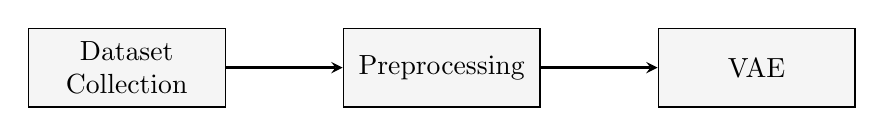
\begin{tikzpicture}[
        node distance=2cm,
        box/.style={rectangle, draw, fill=lightgray, minimum width=2.5cm, minimum height=1cm, align=center},
        arrow/.style={->, >=stealth, thick}
    ]
        \node[box] (data) {Dataset\\Collection};
        \node[box, right of=data, xshift=2cm] (prep) {Preprocessing};
        \node[box, right of=prep, xshift=2cm] (model) {VAE};
        
        \draw[arrow] (data) -- (prep);
        \draw[arrow] (prep) -- (model);
    \end{tikzpicture}
    
    \vspace{0.5cm}
    \begin{keypoint}
    Systematic workflow from data collection through preprocessing to VAE model
    \end{keypoint}
\end{frame}

% --- SLIDE 10: Dataset Collection ---
\begin{frame}{Dataset Collection}
    \textbf{Automated Generation Pipeline:}
    
    \vspace{0.3cm}
    \begin{columns}
        \column{0.52\textwidth}
        \textbf{Font Rendering:}
        \begin{itemize}
            \item PIL/Pillow at 300 DPI
            \item Unicode character mapping
            \item White background, black text
        \end{itemize}
        
        \vspace{0.3cm}
        \textbf{Affine Transformations:}
        \begin{itemize}
            \item \textbf{Size:} 10pt, 14pt, 18pt, 22pt
            \item \textbf{Rotation:} $\pm 3°$
            \item \textbf{Translation:} $\pm 3$ pixels
            \item \textbf{Scaling:} 94\%–106\%
            \item \textbf{Stroke:} Erosion/dilation
        \end{itemize}
        
        \column{0.45\textwidth}
        \textbf{Quality Assessment:}
        \begin{itemize}
            \item SHA-256 hash deduplication
            \item Metadata tracking (JSON)
            \item Automated validation suite
        \end{itemize}
        
        \vspace{0.3cm}
        \begin{keypoint}
        \textbf{Result:} 4,160 images (2,080 per script) with balanced class distribution
        \end{keypoint}
    \end{columns}
\end{frame}

% --- SLIDE 11: Dataset Variations ---
\begin{frame}{Dataset Sample: 9 Variations of 'a' Vowel}
    \centering
    \textbf{Hindi - Akshar Unicode (अ):}
    
    
    \tiny
    \begin{tabular}{ccccccccc}
        \includegraphics[width=0.10\textwidth]{presentation_images/akshar/a_14pt_01.png} &
        \includegraphics[width=0.10\textwidth]{presentation_images/akshar/a_14pt_02.png} &
        \includegraphics[width=0.10\textwidth]{presentation_images/akshar/a_14pt_03.png} &
        \includegraphics[width=0.10\textwidth]{presentation_images/akshar/a_14pt_04.png} &
        \includegraphics[width=0.10\textwidth]{presentation_images/akshar/a_14pt_05.png} &
        \includegraphics[width=0.10\textwidth]{presentation_images/akshar/a_14pt_06.png} &
        \includegraphics[width=0.10\textwidth]{presentation_images/akshar/a_14pt_07.png} &
        \includegraphics[width=0.10\textwidth]{presentation_images/akshar/a_14pt_08.png} &
        \includegraphics[width=0.10\textwidth]{presentation_images/akshar/a_14pt_09.png} \\
        Var 1 & Var 2 & Var 3 & Var 4 & Var 5 & Var 6 & Var 7 & Var 8 & Var 9
    \end{tabular}
    
    \vspace{0.5cm}
    \normalsize
    \textbf{Telugu - Pothana2000 (ఓ):}
    
    \tiny
    \begin{tabular}{ccccccccc}
        \includegraphics[width=0.10\textwidth]{presentation_images/pothana/o_14pt_01.png} &
        \includegraphics[width=0.10\textwidth]{presentation_images/pothana/o_14pt_02.png} &
        \includegraphics[width=0.10\textwidth]{presentation_images/pothana/o_14pt_03.png} &
        \includegraphics[width=0.10\textwidth]{presentation_images/pothana/o_14pt_04.png} &
        \includegraphics[width=0.10\textwidth]{presentation_images/pothana/o_14pt_05.png} &
        \includegraphics[width=0.10\textwidth]{presentation_images/pothana/o_14pt_06.png} &
        \includegraphics[width=0.10\textwidth]{presentation_images/pothana/o_14pt_07.png} &
        \includegraphics[width=0.10\textwidth]{presentation_images/pothana/o_14pt_08.png} &
        \includegraphics[width=0.10\textwidth]{presentation_images/pothana/o_14pt_09.png} \\
        Var 1 & Var 2 & Var 3 & Var 4 & Var 5 & Var 6 & Var 7 & Var 8 & Var 9
    \end{tabular}
    
    \vspace{0.3cm}
    \begin{keypoint}
    \scriptsize Each variation includes systematic transformations: rotation (±3°), translation (±3px), scaling (94\%–106\%), stroke modifications, and contrast adjustments
    \end{keypoint}
\end{frame}

% --- SLIDE 12: Multi-Font Samples ---
\begin{frame}{Dataset Sample: Multi-Font Vowel Characters}
    \vspace{0.2cm}
    \centering
    \small
    \textbf{Akshar Unicode:} a (अ), ai (ऐ), o (ओ) \quad | \quad \textbf{Mangal:} e (ए), au (औ)
    
    \begin{tabular}{ccccc}
        \includegraphics[width=0.15\textwidth]{presentation_images/akshar/a_14pt_01.png} &
        \includegraphics[width=0.15\textwidth]{presentation_images/akshar/ai_14pt_01.png} &
        \includegraphics[width=0.15\textwidth]{presentation_images/akshar/o_14pt_01.png} &
        \includegraphics[width=0.15\textwidth]{presentation_images/mangal/e_14pt_01.png} &
        \includegraphics[width=0.15\textwidth]{presentation_images/mangal/au_14pt_01.png}
    \end{tabular}
    
    \vspace{0.5cm}
    
    \vspace{0.2cm}
    \textbf{Pothana2000:} ai (ఐ), o (ఓ), au (ఔ) \quad | \quad \textbf{Lohit Telugu:} e (ఏ), i (ఇ)
    
    \begin{tabular}{ccccc}
        \includegraphics[width=0.15\textwidth]{presentation_images/pothana/ai_14pt_01.png} &
        \includegraphics[width=0.15\textwidth]{presentation_images/pothana/o_14pt_01.png} &
        \includegraphics[width=0.15\textwidth]{presentation_images/pothana/au_14pt_01.png} &
        \includegraphics[width=0.15\textwidth]{presentation_images/lohit/e_14pt_01.png} &
        \includegraphics[width=0.15\textwidth]{presentation_images/lohit/i_14pt_01.png}
    \end{tabular}
    
    \vspace{0.3cm}
    \begin{keypoint}
    \scriptsize Demonstrates font-specific rendering differences across 4 fonts (2 per script)
    \end{keypoint}
\end{frame}

% ========================================
% SECTION 4: VAE ARCHITECTURE
% ========================================
\section{VAE Architecture}

% --- SLIDE 13: VAE Theory ---
\begin{frame}{Variational Autoencoder: Mathematical Framework}
    \begin{columns}
        \column{0.50\textwidth}
        \textbf{Core Components:}
        \begin{itemize}
            \item \textbf{Encoder} $q_\phi(z|x)$: \\
            Maps input $x$ to latent distribution $\mathcal{N}(\mu, \sigma^2)$
            
            \item \textbf{Latent Variable} $z$: \\
            Sampled via reparameterization: \\
            $z = \mu + \sigma \odot \epsilon$, \quad $\epsilon \sim \mathcal{N}(0,1)$
            
            \item \textbf{Decoder} $p_\theta(x|z)$: \\
            Reconstructs input from $z$
        \end{itemize}
        
        \column{0.48\textwidth}
        \textbf{Loss Function:}
        \begin{align*}
        \mathcal{L} &= \mathcal{L}_{\text{recon}} + \beta \cdot \mathcal{L}_{\text{KL}} \\[0.3cm]
        \mathcal{L}_{\text{recon}} &= \|x - \hat{x}\|^2 \\[0.2cm]
        \mathcal{L}_{\text{KL}} &= D_{KL}(q_\phi(z|x) \| p(z))
        \end{align*}
        
        \vspace{0.3cm}
        \small
        $\beta$: KL weight balancing reconstruction vs. regularization
    \end{columns}
\end{frame}

% --- SLIDE 14: VAE Architecture Diagram ---
\begin{frame}{VAE Architecture}
    \centering
    \includegraphics[width=0.52\textwidth]{presentation_images/image_0.png}
    
    \vspace{0.05cm}
    \scriptsize
    \textbf{Information Flow:}
    \vspace{-0.05cm}
    \begin{itemize}
        \setlength\itemsep{0.02em}
        \item Input image (128×128×3) → Encoder → $\mu, \sigma$ (latent parameters)
        \item Sampling: $z \sim \mathcal{N}(\mu, \sigma^2)$ using reparameterization trick
        \item Decoder: $z$ → Reconstructed image (128×128×3)
        \item Loss backpropagation updates $\phi$ (encoder) and $\theta$ (decoder)
    \end{itemize}
\end{frame}

% ========================================
% SECTION 5: EVALUATION PLAN
% ========================================
\section{Evaluation}

% --- SLIDE 15: Evaluation Metrics ---
\begin{frame}{Evaluation Strategy}
    \begin{columns}
        \column{0.48\textwidth}
        \textbf{Objective Analysis:}
        \begin{itemize}
            \item \textbf{Reconstruction Metrics:} MSE Loss, SSIM
            \item \textbf{Regularization Metrics:} KL Divergence
            \item \textbf{Recognition-Based Validation:} Classification accuracy of generated samples
            \item \textbf{Latent Space Analysis:} t-SNE visualization, Interpolation smoothness
        \end{itemize}
        
        \column{0.48\textwidth}
        \textbf{Subjective Analysis:}
        \begin{itemize}
            \item \textbf{Human Evaluation:} Expert linguist assessment
            \item \textbf{Visual Quality:} Native script readers evaluation
            \item \textbf{Naturalness Scoring:} Character recognizability (1-5 scale)
            \item \textbf{Morphological Correctness:} Stroke smoothness judgment
            \item \textbf{User Studies:} Generated vs. real discrimination test
        \end{itemize}
    \end{columns}
\end{frame}

% ========================================
% SECTION 6: PROGRESS & ROADMAP
% ========================================
\section{Present Work \& Future Work Plan}

% --- SLIDE 16: Work Completed ---
\begin{frame}{Present Work}
    \textbf{Work Completed:}
    \begin{itemize}
        \setlength\itemsep{0.8em}
        \item Literature review on VAEs and Indic script generation
        \item Dataset design and specifications for Telugu and Hindi vowels
        \item Automated generation pipeline implementation
        \item 4,160 images generated across 4 fonts
        \item Quality validation and metadata documentation
        \item VAE architecture design and implementation
    \end{itemize}
\end{frame}

% --- SLIDE 17: Future Work Plan ---
\begin{frame}{Future Work Plan}
    \textbf{Extended Research Directions:}
    \begin{enumerate}
        \setlength\itemsep{0.8em}
        \item \textbf{Transfer Learning:} Apply learned representations to handwritten character datasets (IIIT-Indic-HW)
        
        \item \textbf{Conditional VAE:} Incorporate font labels for controlled multi-font generation
        
        \item \textbf{Full Alphabet Coverage:} Extend to consonants and conjuncts
        
        \item \textbf{Cross-Lingual Models:} Joint latent space for all variations in each script
    \end{enumerate}
\end{frame}

% ========================================
% SECTION 7: REFERENCES
% ========================================
\section*{References}

% --- SLIDE 18: References ---
\begin{frame}[allowframebreaks]{References}
    \small
    \begin{thebibliography}{99}
        
        \bibitem{kingma2013}
        Kingma, Diederik P., and Max Welling. (2013).
        \newblock \href{https://arxiv.org/abs/1312.6114}{Auto-Encoding Variational Bayes}.
        \newblock \textit{arXiv preprint arXiv:1312.6114}. International Conference on Learning Representations (ICLR) 2014.
        
        \bibitem{sumi2019}
        Sumi, Kazuhisa, Takayuki Horie, and Tomo Miyazaki. (2019).
        \newblock \href{https://arxiv.org/abs/1906.06142}{Modality Conversion of Handwritten Patterns by Cross Variational Autoencoders}.
        \newblock \textit{Proceedings of the 15th International Conference on Document Analysis and Recognition (ICDAR)}, pp. 636-641. IEEE.
        
        \bibitem{wang2021}
        Wang, Shuai, Yangliu Kuai, Zheng Zhang, and Xuetao Zhang. (2021).
        \newblock \href{https://ieeexplore.ieee.org/document/9511404}{Learning VAE with Categorical Labels for Generating Conditional Handwritten Characters}.
        \newblock \textit{2021 International Joint Conference on Neural Networks (IJCNN)}, pp. 1-8. IEEE.
        
        \bibitem{seshadri2012}
        Seshadri, Kavitha, and Anil Sontha. (2012).
        \newblock \href{https://link.springer.com/chapter/10.1007/978-3-642-34478-7_12}{A System for Offline Character Recognition Using Auto-encoder Networks}.
        \newblock \textit{Neural Information Processing: 19th International Conference (ICONIP 2012)}, Doha, Qatar, November 12-15, 2012, Proceedings, Part II 19, pp. 90-97. Springer Berlin Heidelberg.
        
        \framebreak
        
        \bibitem{malakar2024}
        Malakar, Sayantan, Showmik Bhowmik, Ram Sarkar, and Mita Nasipuri. (2024).
        \newblock \href{https://link.springer.com/article/10.1007/s11042-024-18655-5}{HCR-Net: A Deep Learning Based Script Independent Handwritten Character Recognition Network}.
        \newblock \textit{Multimedia Tools and Applications}, Vol. 83, pp. 35913-35939. Springer.
        
        \bibitem{krishnan2021}
        Krishnan, Praveen, and C. V. Jawahar. (2021).
        \newblock \href{https://link.springer.com/chapter/10.1007/978-3-030-86337-1_30}{IIIT-Indic-HW-Words: A Dataset for Indic Handwritten Text Recognition}.
        \newblock \textit{Document Analysis and Recognition–ICDAR 2021: 16th International Conference}, Lausanne, Switzerland, September 5-10, 2021, Proceedings, Part III 16, pp. 444-459. Springer International Publishing.
        
        \bibitem{fukui2022}
        Fukui, Kazuhisa, Takayuki Horie, and Tomo Miyazaki. (2022).
        \newblock \href{https://aclanthology.org/2022.lrec-1.799/}{Handwritten Character Generation using Y-Autoencoder for Recognition Model Training}.
        \newblock \textit{Proceedings of the Language Resources and Evaluation Conference (LREC 2022)}, pp. 7380-7387. European Language Resources Association (ELRA).
        
        \bibitem{liu2019}
        Liu, Chunlei, Chengquan Zhang, Dezhi Peng, and Lianwen Jin. (2019).
        \newblock \href{https://ieeexplore.ieee.org/document/8270100}{The Character Generation in Handwriting Feature Extraction Using VAE}.
        \newblock \textit{2017 14th IAPR International Conference on Document Analysis and Recognition (ICDAR)}, Vol. 1, pp. 1094-1099. IEEE.
        
        \bibitem{lee2024}
        Lee, Hyeonjin, Sungsu Kim, and Sungzoon Cho. (2019).
        \newblock \href{https://link.springer.com/article/10.1007/s11063-018-9894-5}{Discriminative Autoencoder for Feature Extraction: Application to Character Recognition}.
        \newblock \textit{Neural Processing Letters}, Vol. 49, pp. 1723-1745. Springer.
        
    \end{thebibliography}
\end{frame}

% --- SLIDE 19: Thank You ---
\begin{frame}
    \vfill
    \centering
    {\Huge \textbf{Thank You}}
    
    \vspace{1cm}
    {\large Questions \& Discussion}
    
    \vspace{1.5cm}
    \begin{columns}
        \column{0.45\textwidth}
        \centering
        \textbf{Karthik M Sarma} \\
        S20230030385
        
        \column{0.45\textwidth}
        \centering
        \textbf{Rohit Pamidi} \\
        S20230030398
    \end{columns}
    
    \vspace{0.5cm}
    \small
    Guide: Dr. Pavan Kumar Perapu \\
    IIIT Sri City
    \vfill
\end{frame}

\end{document}
